\documentclass[a4paper]{article}

\usepackage[sort]{natbib}
\usepackage{fancyhdr}


% \documentclass[a4paper]{article}

\usepackage[english]{babel}
\usepackage[utf8]{inputenc}
\usepackage{amsmath}
\usepackage{graphicx}
\usepackage[colorinlistoftodos]{todonotes}
\usepackage{hyperref}
\usepackage{booktabs} % To thicken table lines
\usepackage{tablefootnote}
\usepackage{listings}
% \usepackage[numbers]{natbib}

\usepackage{graphicx}
\usepackage{babel,blindtext}

\usepackage{algorithm}
\usepackage[noend]{algpseudocode}


% Uirá packages
\usepackage{algorithm}
\usepackage[noend]{algpseudocode}
\usepackage{booktabs} % To thicken table lines
\usepackage{graphicx}
\usepackage{babel,blindtext}
\usepackage{amsmath}
\usepackage[colorinlistoftodos]{todonotes}
\usepackage{hyperref}
\usepackage{mathtools}
\usepackage{listings}
\usepackage{epstopdf}



% you may include other packages here (next line)
\usepackage{enumitem}



%----- you must not change this -----------------
\oddsidemargin 0.2cm
\topmargin -1.0cm
\textheight 24.0cm
\textwidth 15.25cm
% \parindent=0pt
\parskip 1ex
\renewcommand{\baselinestretch}{1.1}
\pagestyle{fancy}
%----------------------------------------------------



% enter your details here----------------------------------

\lhead{\normalsize \textrm{Navigation}}
\chead{}
\rhead{\normalsize August 23, 2018}
\lfoot{\normalsize \textrm{DRLND - Udacity}}
\cfoot{}
\rfoot{Uirá Caiado}
\setlength{\fboxrule}{4pt}\setlength{\fboxsep}{2ex}
\renewcommand{\headrulewidth}{0.4pt}
\renewcommand{\footrulewidth}{0.4pt}


\begin{document}


%----------------your title below -----------------------------

\begin{center}

{\bf \large {Navigation Using Deep Reinforcement Learning \\ \small Uirá Caiado}}
\end{center}


%---------------- start of document body------------------

% The write up is approximately 1 page (500 words) and includes a summary of the paper (including new techniques introduced), and the key results (if any) that were achieved.


According to \cite{spooner2016}, Reinforcement Learning (RL) is an area of machine learning that studies how a learner, called agent, interacts with an environment in order to maximize some notion of cumulative reward. As pointed out by \cite{mnih2015humanlevel}, to use RL successfully in complex environments, with high-dimensional state space, the agent must derive efficient representations of these inputs and use them to generalize past experience to new situations.

In this project, I trained an agent to navigate in a vast, square world, using Unity Machine Learning Agents Toolkit\footnote{Source: \url{https://github.com/Unity-Technologies/ml-agents}} to design, train, and evaluate different variations of the Deep Reinforcement Learning algorithm. This algorithm was first introduced by \cite{mnih2015humanlevel} and combine RL with a class of artificial neural network known as deep neural network, using it to create a 
deep \textit{Q}-network $Q(s, a; \;\theta)$, with parameters $\theta$, to generalize its the past observations to new ones. $s$ and $a$ stands for state and action. Some variants of the Deep Q-Learning (DQN) were also evaluated, including Double Deep Q-learing (DDQN) \cite{HasseltGS15} and DDQN with prioritized experience replay \cite{SchaulQAS15}.

The environment used for this project is the Udacity version of the Banana Collector environment, from Unity\footnote{Source: \url{https://youtu.be/heVMs3t9qSk}}. The goal of the agent is to collect as many yellow bananas as possible while avoiding blue bananas. The task is episodic, and to solve the environment, the agent must get an average score of +13 over 100 consecutive episodes.

A reward of +1 is provided for collecting a yellow banana, and a reward of -1 is provided for collecting a blue banana. The state space has 37 dimensions and contains the agent’s velocity, along with a ray-based perception of objects around agent’s forward direction. Given this information, the agent has to learn how to best select actions. Four discrete actions are available, corresponding to moving forward, backward, turn left and right.


The first algorithm tested was the vanilla DQN...

\begin{figure}[ht]
\centering
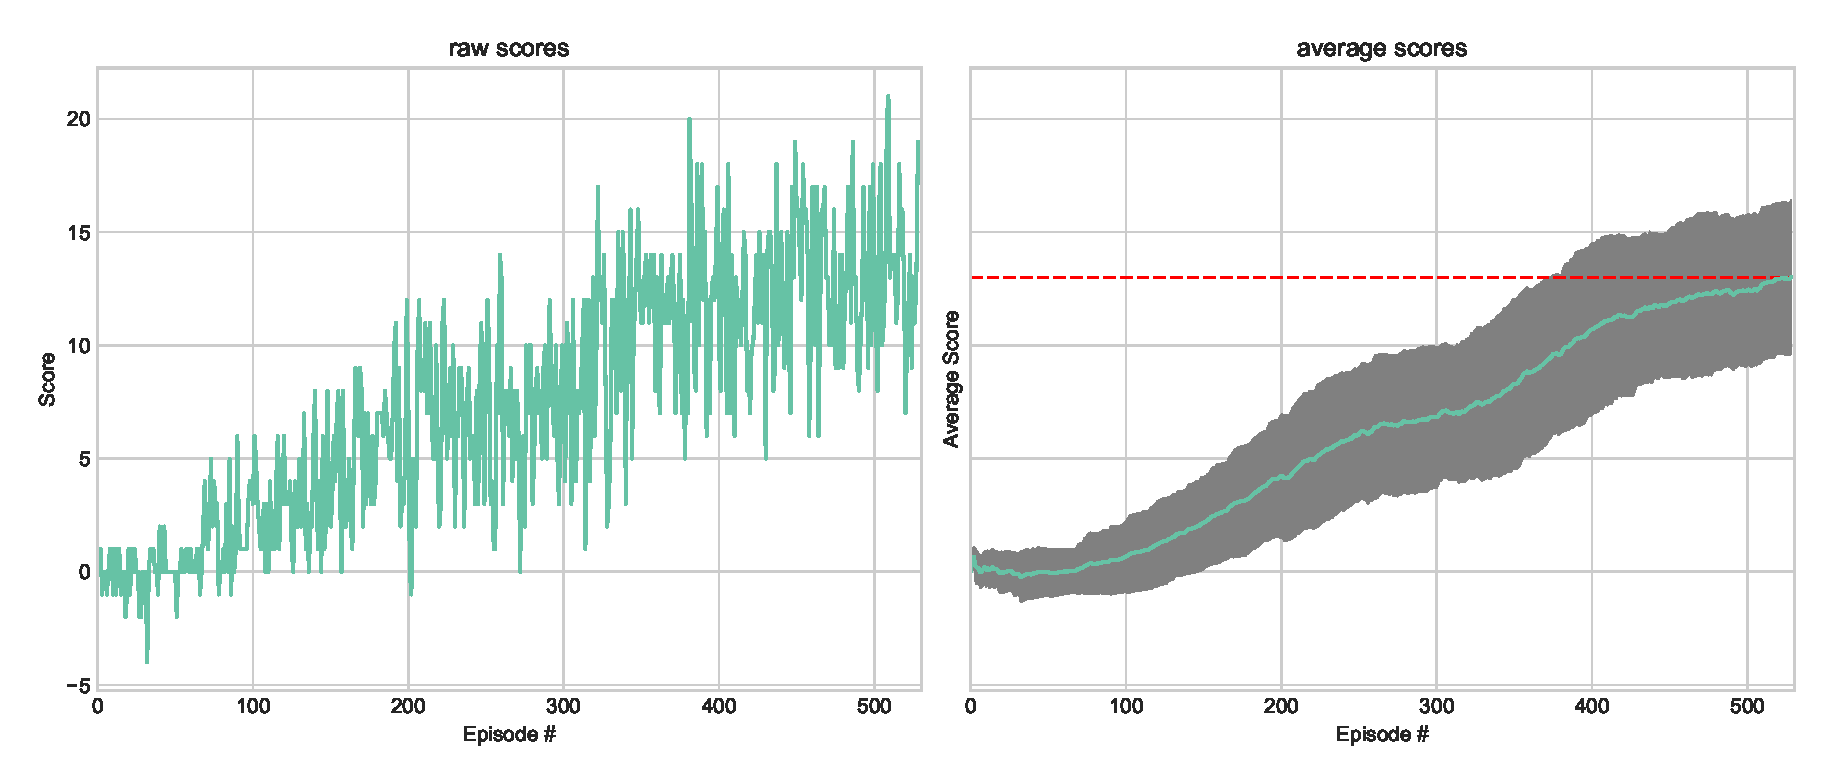
\includegraphics[width=0.7\textwidth]{../notebooks/figures/2018-08-24-dqn.eps}
\caption{Moving Average of $100$ episodes of the score}
\label{fig:dqn}
\end{figure}


The second was the DDQN...

\begin{figure}[ht]
\centering
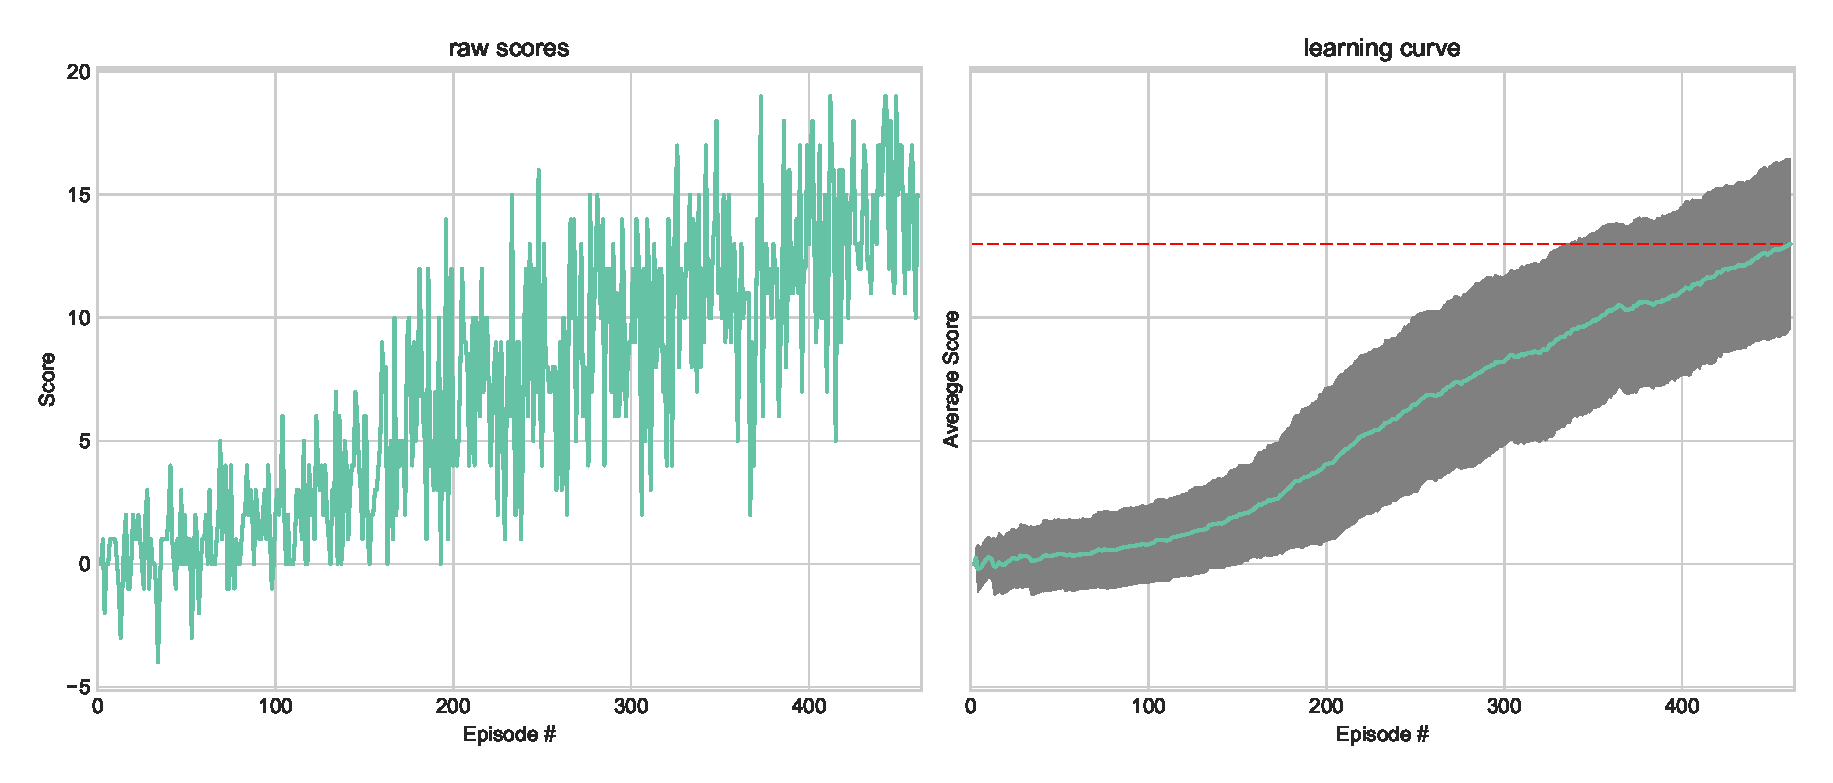
\includegraphics[width=0.7\textwidth]{../notebooks/figures/2018-08-24-ddqn-learning-curve.eps}
\caption{Moving Average of $100$ episodes of the score}
\label{fig:ddqn}
\end{figure}

The last one was the DDQN with prioritized experience replay

bla the figure \ref{fig:ddqnper}

\begin{figure}[ht]
\centering
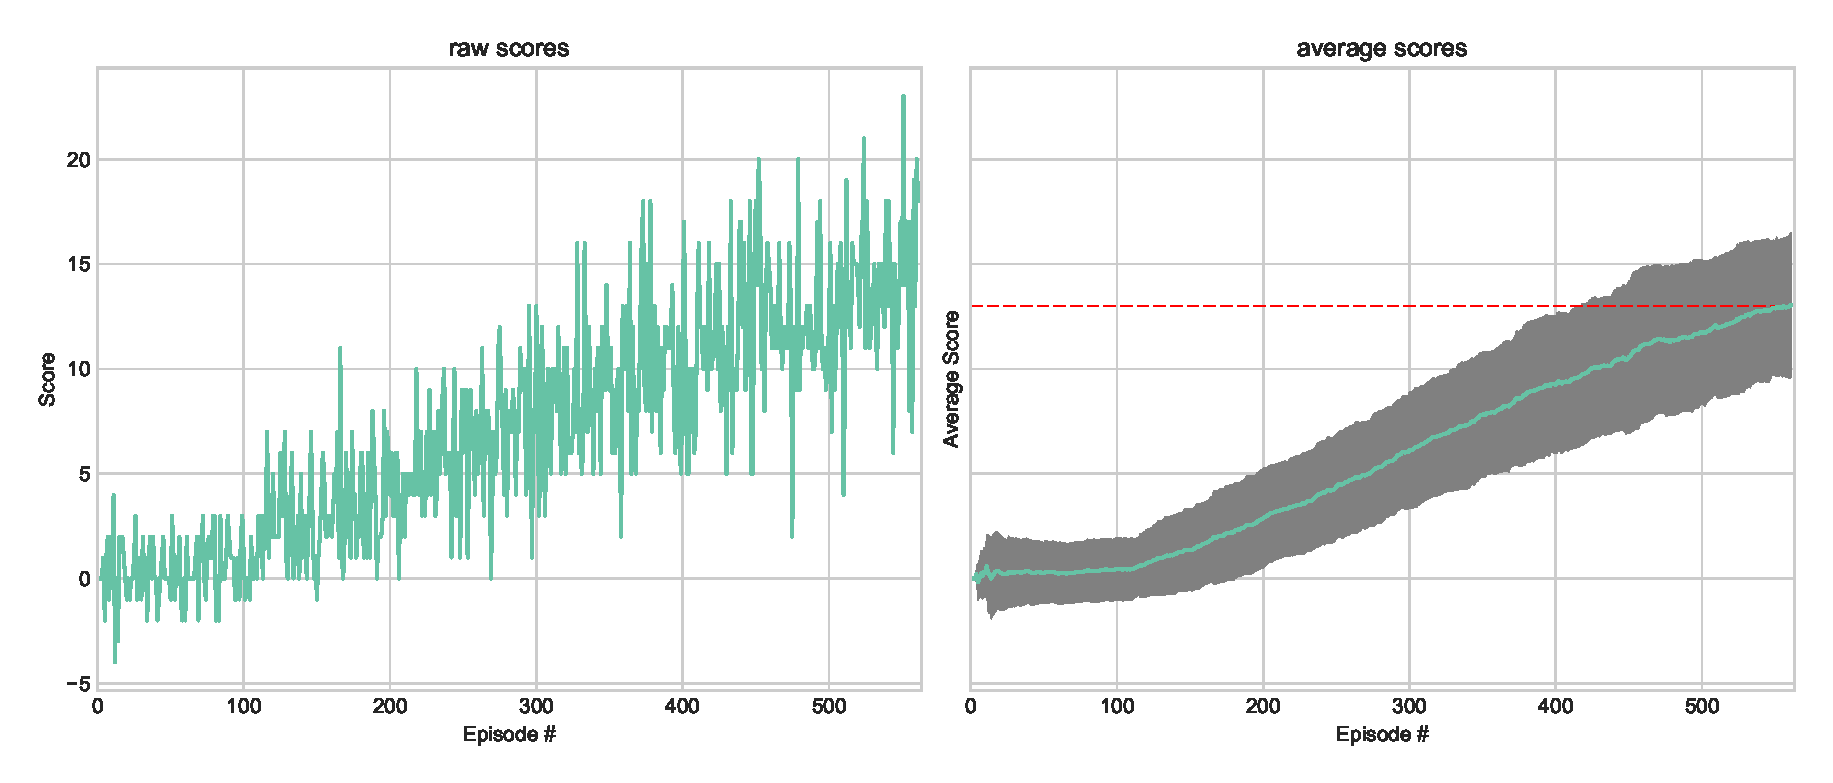
\includegraphics[width=0.7\textwidth]{../notebooks/figures/2018-08-23-ddqnpre-learning-curve.eps}
\caption{Moving Average of $100$ episodes of the score}
\label{fig:ddqnper}
\end{figure}


and bla bla bla

\begin{figure}[ht]
\centering
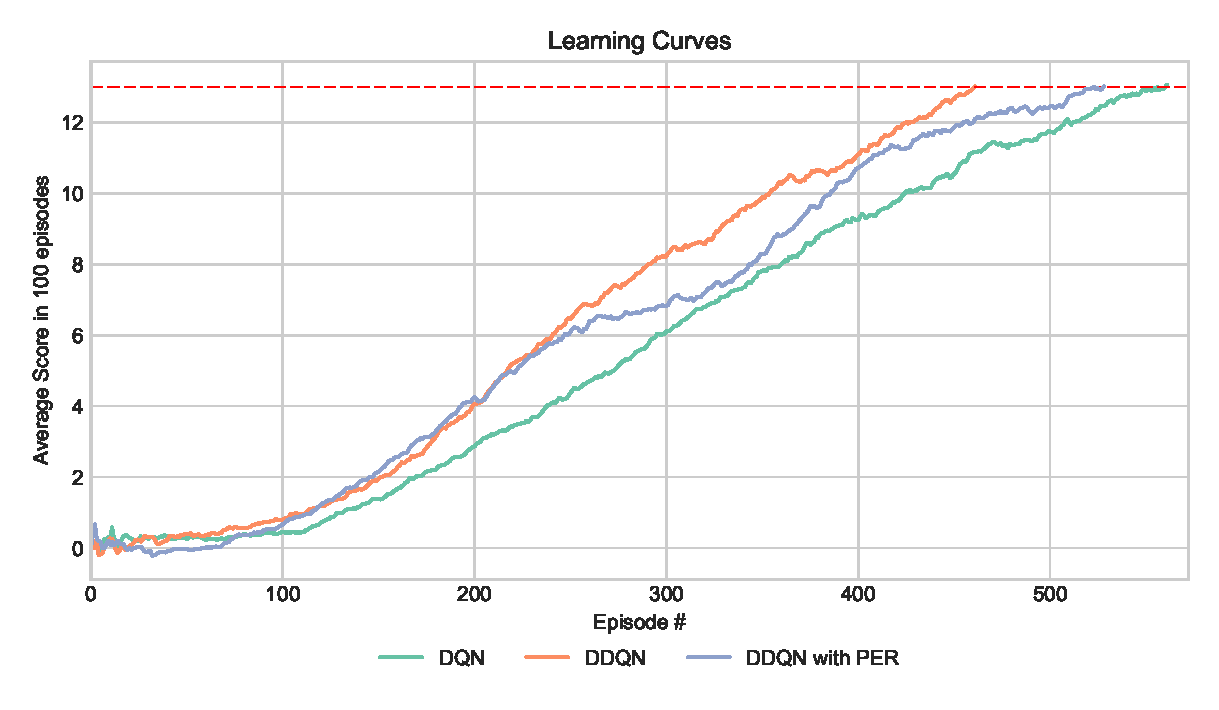
\includegraphics[width=0.7\textwidth]{../notebooks/figures/2018-08-23-final-comparition-2.eps}
\caption{Moving Average of $100$ episodes of the score}
\label{fig:final_comp}
\end{figure}


Finally, as possible extensions ...



% ----------------end of document body---------------------

%---------------- start of references------------------

\bibliographystyle{plain}
% or try abbrvnat or unsrtnat
\bibliography{biblio.bib}

%---------------- end of references------------------


\end{document}
